\documentclass{beamer}
\usepackage[utf8]{inputenc}

\usetheme{Boadilla}
\usecolortheme{lily}
\usepackage{amsmath,amssymb,amsfonts,amsthm}
\usepackage{mathtools}
\usepackage{txfonts}
\usepackage{tkz-euclide}
\usepackage{listings}
\usepackage{adjustbox}
\usepackage{array}
\usepackage{tabularx}
\usepackage{lmodern}
\usepackage{gvv}
\usepackage{circuitikz}
\usepackage{tikz}
\usepackage{graphicx}

\setbeamertemplate{footline}
{
  \leavevmode%
  \hbox{%
  \begin{beamercolorbox}[wd=\paperwidth,ht=2.25ex,dp=1ex,right]{author in head/foot}%
    \insertframenumber{} / \inserttotalframenumber\hspace*{2ex} 
  \end{beamercolorbox}}%
  \vskip0pt%
}

\usepackage{tcolorbox}
\tcbuselibrary{minted,breakable,xparse,skins}




\providecommand{\nCr}[2]{\,^{#1}C_{#2}} % nCr
\providecommand{\nPr}[2]{\,^{#1}P_{#2}} % nPr
\providecommand{\mbf}{\mathbf}
\providecommand{\pr}[1]{\ensuremath{\Pr\left(#1\right)}}
\providecommand{\qfunc}[1]{\ensuremath{Q\left(#1\right)}}
\providecommand{\sbrak}[1]{\ensuremath{{}\left[#1\right]}}
\providecommand{\lsbrak}[1]{\ensuremath{{}\left[#1\right.}}
\providecommand{\rsbrak}[1]{\ensuremath{{}\left.#1\right]}}
\providecommand{\brak}[1]{\ensuremath{\left(#1\right)}}
\providecommand{\lbrak}[1]{\ensuremath{\left(#1\right.}}
\providecommand{\rbrak}[1]{\ensuremath{\left.#1\right)}}
\providecommand{\cbrak}[1]{\ensuremath{\left\{#1\right\}}}
\providecommand{\lcbrak}[1]{\ensuremath{\left\{#1\right.}}
\providecommand{\rcbrak}[1]{\ensuremath{\left.#1\right\}}}
\theoremstyle{remark}
\newcommand{\sgn}{\mathop{\mathrm{sgn}}}
\providecommand{\abs}[1]{\left\vert#1\right\vert}
\providecommand{\res}[1]{\Res\displaylimits_{#1}} 
\providecommand{\norm}[1]{\lVert#1\rVert}
\providecommand{\mtx}[1]{\mathbf{#1}}
\providecommand{\mean}[1]{E\left[ #1 \right]}
\providecommand{\fourier}{\overset{\mathcal{F}}{ \rightleftharpoons}}
%\providecommand{\hilbert}{\overset{\mathcal{H}}{ \rightleftharpoons}}
\providecommand{\system}{\overset{\mathcal{H}}{ \longleftrightarrow}}
	%\newcommand{\solution}[2]{\textbf{Solution:}{#1}}
%\newcommand{\solution}{\noindent \textbf{Solution: }}
\providecommand{\dec}[2]{\ensuremath{\overset{#1}{\underset{#2}{\gtrless}}}}
\newcommand{\myvec}[1]{\ensuremath{\begin{pmatrix}#1\end{pmatrix}}}
\let\vec\mathbf

\lstset{
%language=C,
frame=single, 
breaklines=true,
columns=fullflexible
}

\numberwithin{equation}{section}

\lstset{
  language=Python,
  basicstyle=\ttfamily\small,
  keywordstyle=\color{blue},
  stringstyle=\color{orange},
  numbers=left,
  numberstyle=\tiny\color{gray},
  breaklines=true,
  showstringspaces=false
}

\title{Problem 1.1.23}
\author{ee25btech11023-Venkata Sai}

\date{\today} 
\begin{document}

\begin{frame}
\titlepage
\end{frame}

\section*{Outline}
\begin{frame}
\tableofcontents
\end{frame}

\section{Problem}

\begin{frame}
\frametitle{Problem}
A unity feedback control system has an open-loop transfer function 
\begin{align}
G(s) = \frac{K}{s(s^2 + 7s + 12)}.
\end{align}
The gain $K$ for which $s = -1 + j1$ will lie on the root locus of this system is: \hfill(EC 2007)


\begin{enumerate}
    \item 4 
    \item 5.5
    \item 6.5
    \item 10 
\end{enumerate}
\end{frame}
%\subsection{Literature}
\section{Solution}

\subsection{Formula}
\setcounter{section}{1}
\begin{frame}
\frametitle{Formula}
We define the open-loop transfer function as
\begin{align}
    G(s) = K \cdot P(s)
\end{align}
where P(s) is called Plant and K is called Gain
\begin{align}
    P(s) = \frac{1}{s(s^2 + 7s + 12)}=\frac{1}{s(s+3)(s+4)}
\end{align}
In control theory, a point $s$ lies on the root locus if it satisfies the characteristic equation:
\begin{align}
1 + G(s)H(s) = 0 &\implies 1 + KP(s)H(s) = 0\\
KP(&s)H(s)=-1 \\
|KP(&s)H(s)| = 1  
\end{align}
For an unity feedback system , $H(s)$ equals 1. Then,
\begin{align}
    |KP(s)| = 1  
\end{align}

\end{frame}
\subsection{Calculation}
\begin{frame}
\frametitle{Calculation}
In Root Locus analysis, the gain K is assumed to be a positive real number (K$>$0). So,
\begin{align}
   K|P(s)| = 1  \implies K=\frac{1}{|P(s)|}
\end{align}
From (1.2)
\begin{align}
    K=|s(s+3)(s+4)|  
    \end{align}
    On substituting $s=-1+j1$,
    \begin{align}
    K&= |(-1+j1)(-1+j1+3)(-1+j1+4)| \\
    K&= |(-1+j1)(2+j1)(3+j1)| \\
    K&= \brak{\sqrt{1^2+1^2}}\brak{\sqrt{2^2+1^2}}\brak{\sqrt{3^2+1^2}}\\
   K&= \brak{\sqrt{2}}\brak{\sqrt{5}}\brak{\sqrt{10}} = \sqrt{100} =10
\end{align}
Hence the value of $K$ is 10.
\end{frame}

\begin{frame}
\frametitle{Calculation}
 \begin{align}
     G(s) = \frac{K}{s(s^2 + 7s + 12)} = \frac{K}{s(s+3)(s+4)}
 \end{align}
 To find open-loop poles, we make the denominator = 0
 \begin{align}
     s(s+3)(s+4)=0
 \end{align}
 Hence, the open-loop poles are 0,-3,-4
 
 After applying the feedback, the closed loop poles are the roots of 
 \begin{align}
     1+G(s)H(s)=0 \\
     1+ \frac{K}{s(s+3)(s+4)} = 0  \\
     s^3 + 7s^2 + 12s + K =0 
 \end{align}
 When K=10, the roots are $-1 \pm j1 $ and -5 . These are called closed loop poles.
 \end{frame}

\section{Plot}

\begin{frame}
\frametitle{Plot}
\begin{figure}
    \centering
    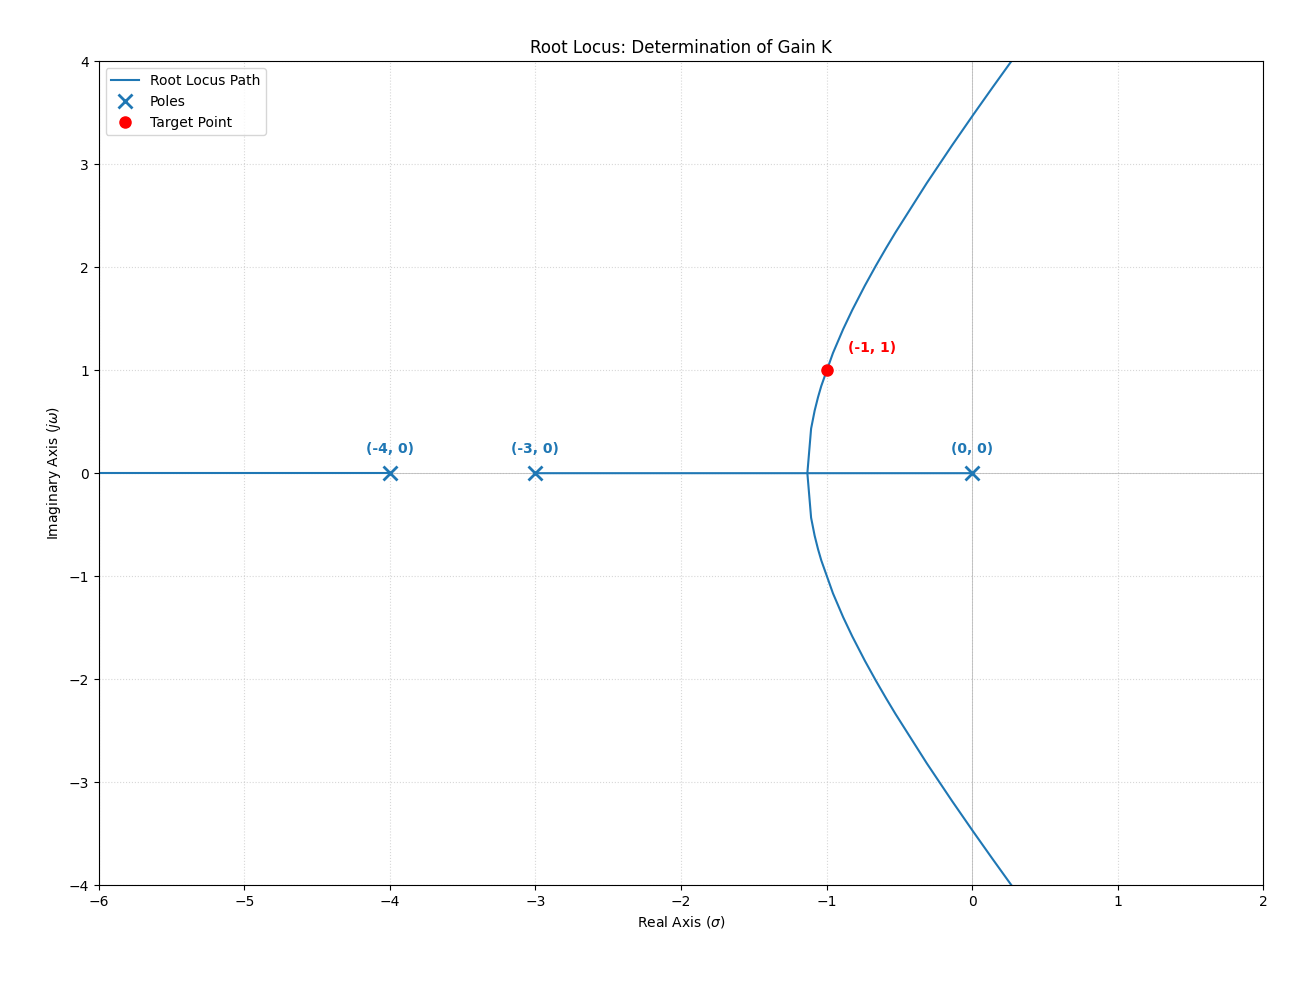
\includegraphics[width=0.9\linewidth]{figs/fig1.png}
    \label{Figure 1}
\end{figure}
\end{frame}

\section{Python Code}
\begin{frame}[fragile]
\frametitle{Python Code for Plotting}
\begin{lstlisting}[language=Python]
import numpy as np
import control as ct
import matplotlib.pyplot as plt

# G(s) = K / [s(s+3)(s+4)]
num = [1]
den = [1, 7, 12, 0] # s^3 + 7s^2 + 12s
sys = ct.TransferFunction(num, den)

# Find poles
s_target = -1 + 1j
poles = ct.poles(sys)

# K = Product of distances from each pole to the target point
distances = [np.abs(s_target - p) for p in poles]
K_calc = np.prod(distances)

# Visualization
plt.figure(figsize=(9, 6))


\end{lstlisting}
\end{frame}
 
\begin{frame}[fragile]
\frametitle{Python Code for Plotting}
\begin{lstlisting}[language=Python]
# Root Locus
roots, gains = ct.root_locus(sys, plot=False)

# Plot Root Locus Path
for i in range(roots.shape[1]):
    lbl = 'Root Locus Path' if i == 0 else ""
    plt.plot(np.real(roots[:, i]), np.imag(roots[:, i]), color='C0', lw=1.5, label=lbl, zorder=2)

# Plot Open-Loop Poles
plt.plot(np.real(poles), np.imag(poles), 'x', color='C0', markersize=10, mew=2, label='Poles', zorder=3)

# Plot Target Point
plt.plot(s_target.real, s_target.imag, 'ro', markersize=8, label=f'Target Point', zorder=4)


\end{lstlisting}
\end{frame}
\begin{frame}[fragile]
\frametitle{Python Code for Plotting}
\begin{lstlisting}[language=Python]
for p in poles:
    x_coord = np.real(p)
    y_coord = np.imag(p)
    # Using :g formats it cleanly without trailing zeros
    plt.text(x_coord, y_coord + 0.2, f'({x_coord:g}, {y_coord:g})',
             color='C0', fontsize=10, fontweight='bold', ha='center')

t_x = s_target.real
t_y = s_target.imag
plt.text(t_x + 0.15, t_y + 0.15, f'({t_x:g}, {t_y:g})',
         color='red', fontsize=10, fontweight='bold', va='bottom', ha='left')

plt.title("Root Locus: Determination of Gain K")
plt.xlabel("Real Axis ($\sigma$)")


\end{lstlisting}
\end{frame}
\begin{frame}[fragile]
\frametitle{Python Code for Plotting}
\begin{lstlisting}[language=Python]
plt.ylabel("Imaginary Axis ($j\omega$)")
plt.axhline(0, color='black', lw=0.5, alpha=0.3, zorder=1)
plt.axvline(0, color='black', lw=0.5, alpha=0.3, zorder=1)
plt.grid(True, linestyle=':', alpha=0.5)
plt.xlim([-6, 2])
plt.ylim([-4, 4])
plt.legend(loc='upper left')
plt.tight_layout()
plt.show()

print(f"Target Point Coordinates: ({s_target.real:g}, {s_target.imag:g})")
print(f"Pole Coordinates: {[(np.real(p), np.imag(p)) for p in poles]}")
print(f"Calculated Gain K: {K_calc:.2f}")
\end{lstlisting}
\end{frame}

\end{document}
